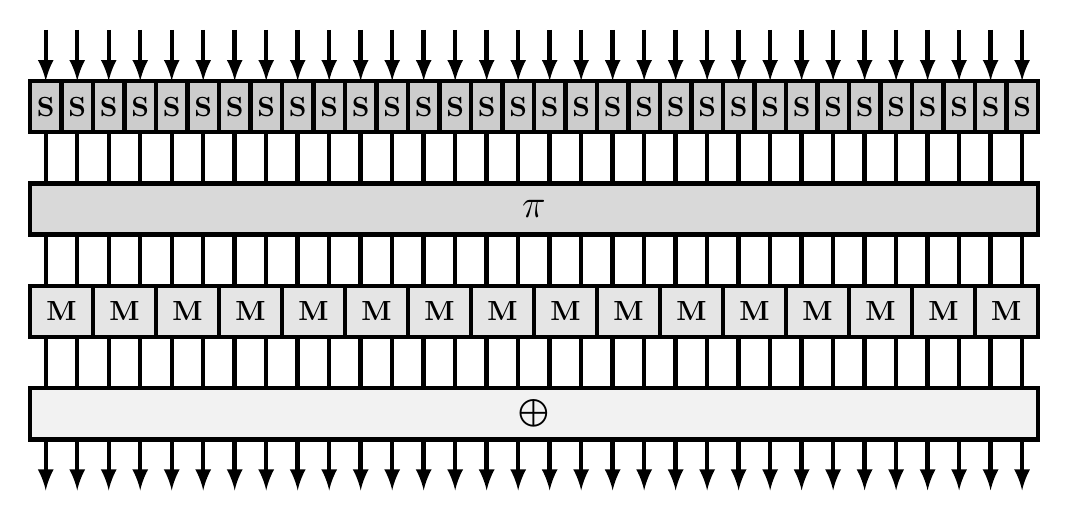
\begin{tikzpicture}[xscale=0.4,yscale=0.65,>=latex,ultra thick]
% Reference grid (temporary)
%\draw[help lines] (0,0) grid (32,32);

% TODO label bits / words

% Entry arrows
\foreach \i in {32,...,1} {
  \draw[->] (\i-0.5,32) -- (\i-0.5, 31);
}

% S-boxes
\foreach \i in {32,...,1} {
  \draw[fill=gray!40] (\i,30) rectangle (\i-1,31) node[midway] {$\mathbf{S}$} ;
}

% P-boxes
\draw[fill=gray!30] (0,28) rectangle (32,29) node[midway] {\Large$\mathbf{\pi}$};

% Wires
\foreach \j in {25,27,29} {
  \foreach \i in {32,...,1} {
    \draw (\i-0.5,\j) -- (\i-0.5,\j+1);
  }
}

% Mixers
\foreach \i in {2,4,...,32} {
  \draw[fill=gray!20] (\i,26) rectangle (\i-2,27) node[midway] {$\mathbf{M}$};
}

% Round key box
\draw[fill=gray!10] (0,24) rectangle (32,25) node[midway] {$\bigoplus$};
%\foreach \i in {32,...,1} {
  %\draw[fill=gray!15,line width=2.5pt] (#1, #2) ellipse (1em and 1em);
  %\draw[line width=2.5pt] (#1-.4, #2) -- (#1+.4, #2);
  %\draw[line width=2.5pt] (#1, #2-.4) -- (#1, #2+.4);
%}

% Exit arrows
\foreach \i in {32,...,1} {
  \draw[->] (\i-0.5,24) -- (\i-0.5, 23);
}

\end{tikzpicture}

